\documentclass[border=4pt]{standalone}
\usepackage{unicode-math}
\setmainfont{TeX Gyre Termes}
\setmathfont{TeX Gyre Termes Math}
\usepackage{tikz}
\usetikzlibrary{arrows.meta,positioning,calc,decorations.pathreplacing}
\usepackage{pgfplots}
\pgfplotsset{compat=1.18}
\definecolor{elemA}{HTML}{1F5FA8}
\definecolor{elemB}{HTML}{B8461B}
\definecolor{elemC}{HTML}{2E7D32}
\definecolor{elemD}{HTML}{6A4C93}
\definecolor{frameline}{HTML}{555555}

\usetikzlibrary{decorations.pathmorphing,patterns}
\begin{document}
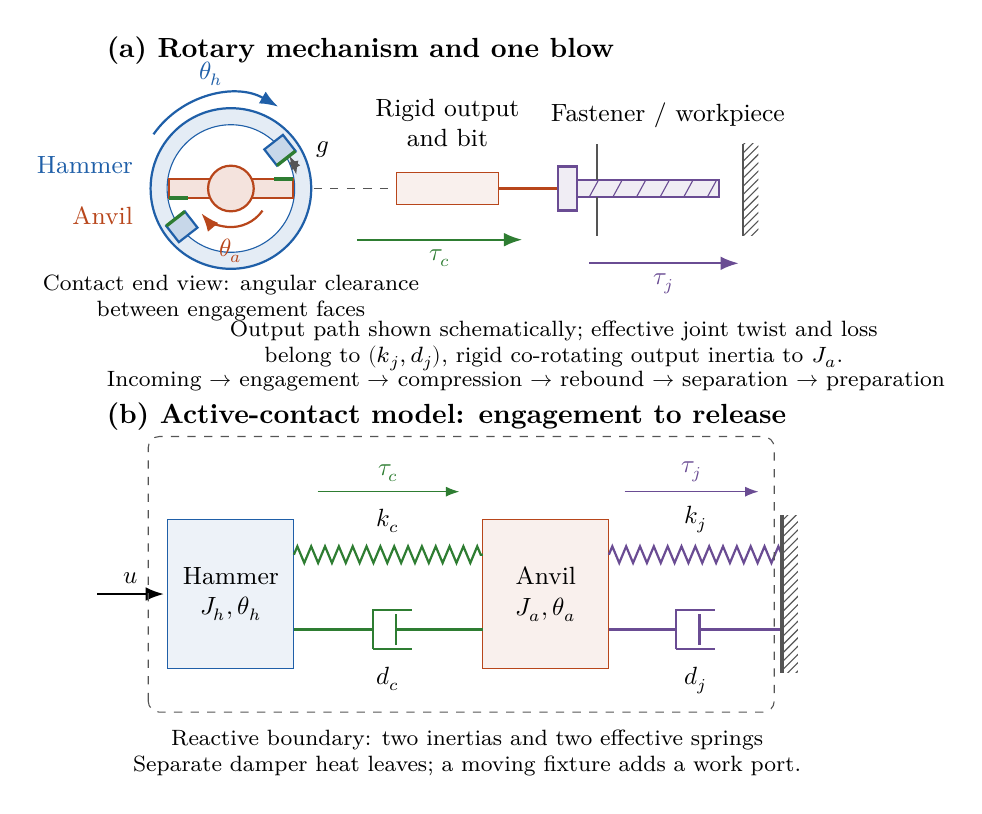
\begin{tikzpicture}[>=Latex,font=\small]
% Contact end view and a schematic output path; not a manufacturing drawing.
\node[anchor=west,font=\bfseries] at (-1.7,6.9) {(a) Rotary mechanism and one blow};
\begin{scope}[shift={(0,5.15)}]
  \fill[elemA!12,even odd rule] (0,0) circle (1.02) (0,0) circle (.81);
  \draw[elemA,thick] (0,0) circle (1.02);
  \draw[elemA] (0,0) circle (.81);
  \foreach \ang in {38,218} {
    \begin{scope}[rotate=\ang]
      \filldraw[fill=elemA!25,draw=elemA,thick] (.64,-.13) rectangle (.94,.13);
      \draw[elemC,very thick] (.64,-.13)--(.94,-.13);
    \end{scope}
  }
  \filldraw[draw=elemB,fill=elemB!15,thick] (-.79,-.12) rectangle (.79,.12);
  \filldraw[draw=elemB,fill=elemB!15,thick] (0,0) circle (.29);
  \draw[elemC,very thick] (.55,.12)--(.79,.12);
  \draw[elemC,very thick] (-.55,-.12)--(-.79,-.12);
  \draw[<->,frameline] (12:.85) arc[start angle=12,end angle=29,radius=.85];
  \node[anchor=west] at (.96,.5) {$g$};
  \draw[->,elemA,thick] (145:1.2) arc[start angle=145,end angle=60,radius=1.2];
  \node[above,elemA] at (-.25,1.18) {$\theta_h$};
  \draw[->,elemB,thick] (-35:.49) arc[start angle=-35,end angle=-140,radius=.49];
  \node[below,elemB] at (0,-.51) {$\theta_a$};
  \node[anchor=east,align=right,elemA] at (-1.12,.3) {Hammer};
  \node[anchor=east,align=right,elemB] at (-1.12,-.35) {Anvil};
\end{scope}
\node[align=center,font=\footnotesize] at (0,3.76) {Contact end view: angular clearance\\between engagement faces};
\draw[dashed,frameline] (1.05,5.15)--(2.05,5.15);
\node[draw=elemB,fill=elemB!8,minimum width=1.3cm,minimum height=.4cm] (bit) at (2.75,5.15) {};
\node[above,align=center] at (2.75,5.55) {Rigid output\\and bit};
\draw[elemB,thick] (3.4,5.15)--(4.15,5.15);
\draw[elemD,thick,fill=elemD!10] (4.15,4.87) rectangle (4.4,5.43);
\draw[elemD,thick,fill=elemD!10] (4.4,5.04) rectangle (6.2,5.26);
\foreach \x in {4.55,4.85,5.15,5.45,5.75,6.05}
  \draw[elemD] (\x,5.04)--(\x+.12,5.26);
\draw[frameline,thick] (4.65,4.55)--(4.65,5.04) (4.65,5.26)--(4.65,5.72);
\draw[frameline,thick] (6.5,4.55)--(6.5,5.72);
\fill[pattern=north east lines,pattern color=frameline] (6.5,4.55) rectangle (6.7,5.72);
\node[above,align=center] at (5.55,5.8) {Fastener / workpiece};
\draw[->,elemC,thick] (1.6,4.5)--(3.7,4.5) node[midway,below] {$\tau_c$};
\draw[->,elemD,thick] (4.55,4.2)--(6.45,4.2) node[midway,below] {$\tau_j$};
\node[font=\footnotesize,align=center] at (4.1,3.15) {Output path shown schematically; effective joint twist and loss\\belong to $(k_j,d_j)$, rigid co-rotating output inertia to $J_a$.};
\node[anchor=west,font=\footnotesize] at (-1.7,2.7) {Incoming $\to$ engagement $\to$ compression $\to$ rebound $\to$ separation $\to$ preparation};
\node[anchor=west,font=\bfseries] at (-1.7,2.25) {(b) Active-contact model: engagement to release};
\node[draw=elemA,fill=elemA!8,minimum width=1.6cm,minimum height=1.9cm,align=center] (h) at (0,0) {Hammer\\$J_h,\theta_h$};
\node[draw=elemB,fill=elemB!8,minimum width=1.6cm,minimum height=1.9cm,align=center] (a) at (4,0) {Anvil\\$J_a,\theta_a$};
\draw[decorate,decoration={zigzag,segment length=5pt,amplitude=3pt},elemC,thick] (.8,.5)--(3.2,.5);
\node[above] at (2,.65) {$k_c$};
\draw[elemC,thick] (.8,-.45)--(1.8,-.45);
\draw[elemC,thick] (1.8,-.7)--(1.8,-.2)--(2.3,-.2);
\draw[elemC,thick] (1.8,-.7)--(2.3,-.7);
\draw[elemC,thick] (2.1,-.65)--(2.1,-.25);
\draw[elemC,thick] (2.1,-.45)--(3.2,-.45);
\node[below] at (2,-.8) {$d_c$};
\draw[decorate,decoration={zigzag,segment length=5pt,amplitude=3pt},elemD,thick] (4.8,.5)--(7,.5);
\node[above] at (5.9,.65) {$k_j$};
\draw[elemD,thick] (4.8,-.45)--(5.65,-.45);
\draw[elemD,thick] (5.65,-.7)--(5.65,-.2)--(6.15,-.2);
\draw[elemD,thick] (5.65,-.7)--(6.15,-.7);
\draw[elemD,thick] (5.95,-.65)--(5.95,-.25);
\draw[elemD,thick] (5.95,-.45)--(7,-.45);
\node[below] at (5.9,-.8) {$d_j$};
\draw[frameline,very thick] (7,-1)--(7,1);
\fill[pattern=north east lines,pattern color=frameline] (7,-1) rectangle (7.2,1);
\draw[->,thick] (-1.7,0)--(-.85,0) node[midway,above] {$u$};
\draw[->,elemC] (1.1,1.3)--(2.9,1.3) node[midway,above] {$\tau_c$};
\draw[->,elemD] (5,1.3)--(6.7,1.3) node[midway,above] {$\tau_j$};
\draw[dashed,rounded corners,frameline] (-1.05,-1.5) rectangle (6.9,2);
\node[below,align=center,font=\footnotesize] at (3,-1.6) {Reactive boundary: two inertias and two effective springs\\Separate damper heat leaves; a moving fixture adds a work port.};
\end{tikzpicture}
\end{document}
